\section{Referencia de la Estructura ast}
\label{structast}\index{ast@{ast}}
Estructura del arbol abstracto de sintaxis (AST), basico para poder evaluar construcciones iterativas del lenguaje.  


{\tt \#include $<$ast.h$>$}

Diagrama de colaboraci\'{o}n para ast:\begin{figure}[H]
\begin{center}
\leavevmode
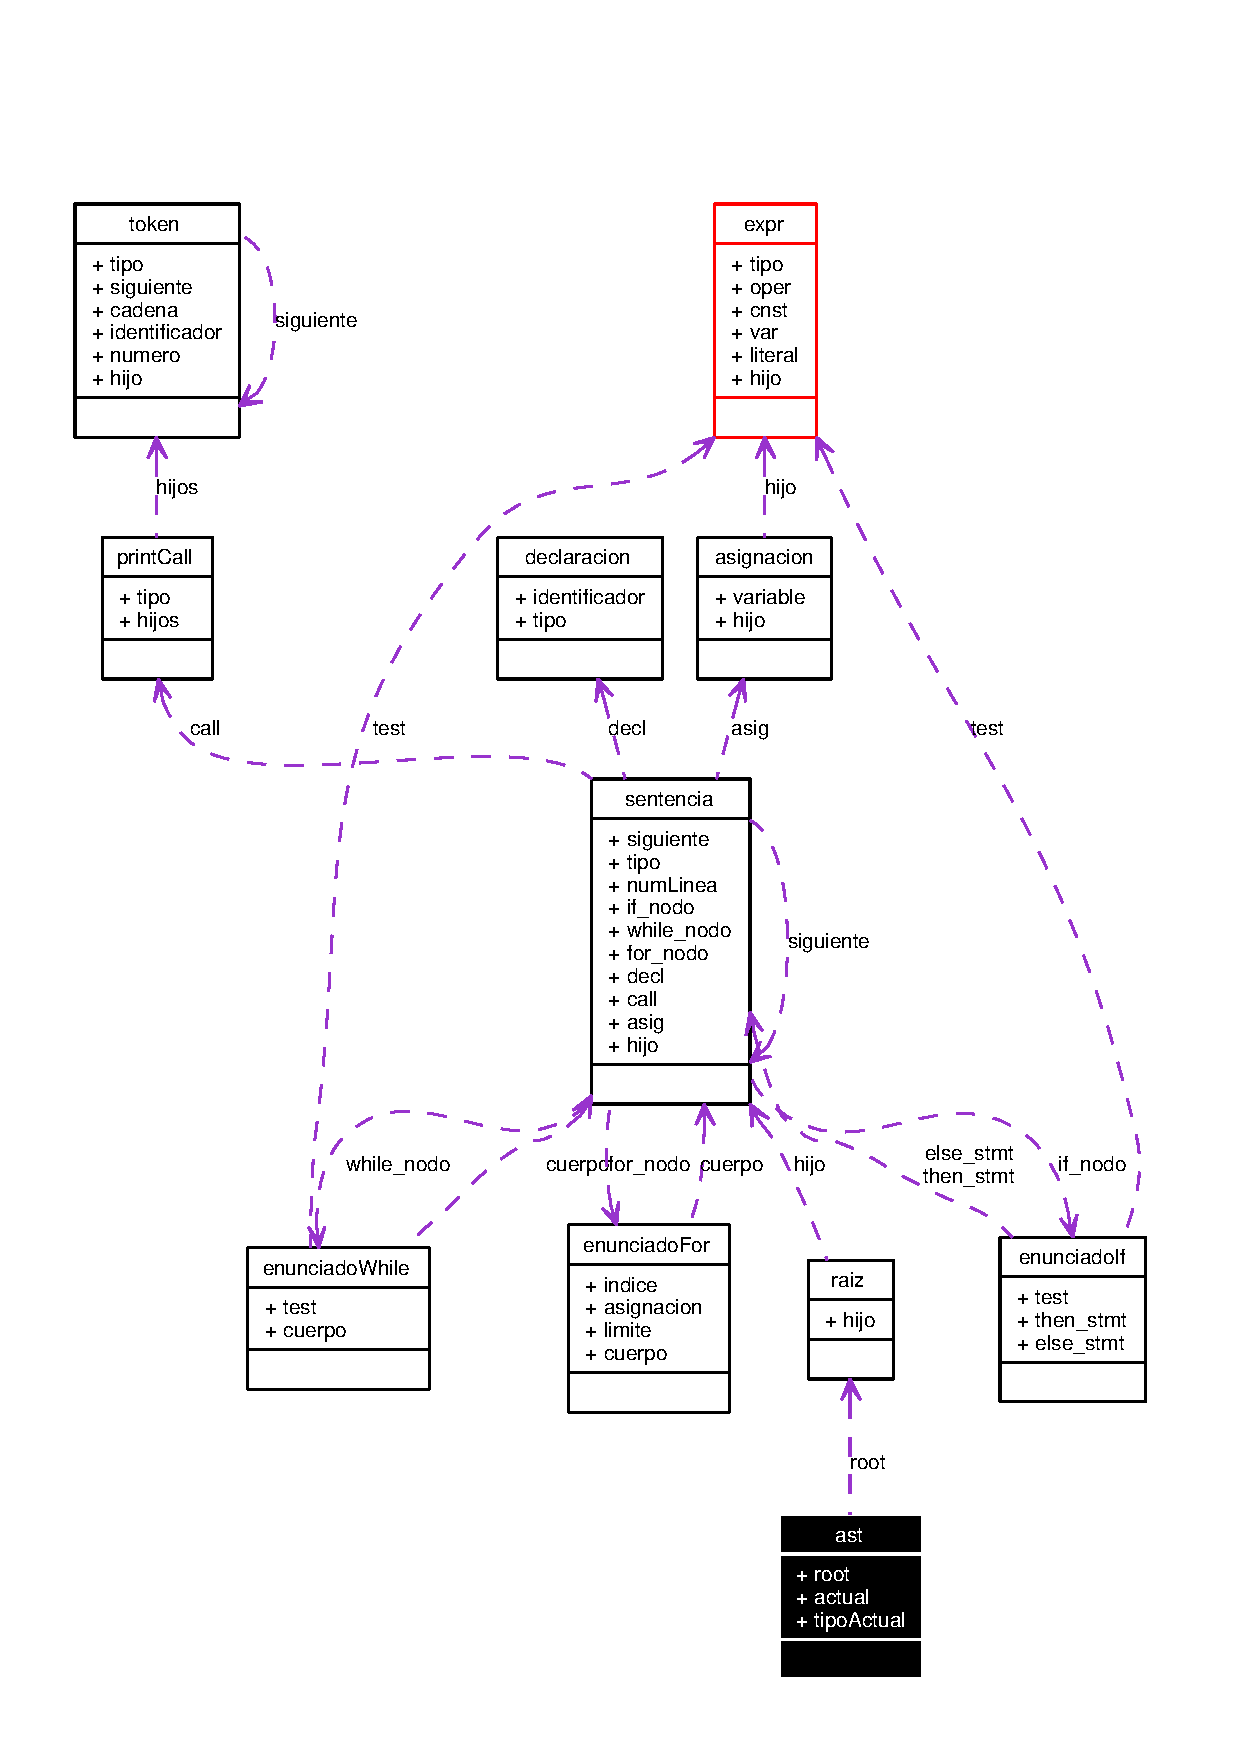
\includegraphics[width=290pt]{structast__coll__graph}
\end{center}
\end{figure}
\subsection*{Atributos p\'{u}blicos}
\begin{CompactItemize}
\item 
{\bf raiz} $\ast$ {\bf root}
\begin{CompactList}\small\item\em apuntador a raiz \item\end{CompactList}\item 
void $\ast$ {\bf actual}
\begin{CompactList}\small\item\em puntero auzliiar \item\end{CompactList}\item 
int {\bf tipo\-Actual}
\begin{CompactList}\small\item\em tipo del nodo actual \item\end{CompactList}\end{CompactItemize}


\subsection{Descripci\'{o}n detallada}
Estructura del arbol abstracto de sintaxis (AST), basico para poder evaluar construcciones iterativas del lenguaje. 



Definici\'{o}n en la l\'{\i}nea 268 del archivo ast.h.

\subsection{Documentaci\'{o}n de los datos miembro}
\index{ast@{ast}!actual@{actual}}
\index{actual@{actual}!ast@{ast}}
\subsubsection{\setlength{\rightskip}{0pt plus 5cm}void$\ast$ {\bf ast::actual}}\label{structast_o1}


puntero auzliiar 



Definici\'{o}n en la l\'{\i}nea 270 del archivo ast.h.

Referenciado por borrar\-Arbol(), y crear\-Raiz().\index{ast@{ast}!root@{root}}
\index{root@{root}!ast@{ast}}
\subsubsection{\setlength{\rightskip}{0pt plus 5cm}{\bf raiz}$\ast$ {\bf ast::root}}\label{structast_o0}


apuntador a raiz 



Definici\'{o}n en la l\'{\i}nea 269 del archivo ast.h.

Referenciado por borrar\-Arbol(), crear\-Raiz(), y recorrer\-Arbol().\index{ast@{ast}!tipoActual@{tipoActual}}
\index{tipoActual@{tipoActual}!ast@{ast}}
\subsubsection{\setlength{\rightskip}{0pt plus 5cm}int {\bf ast::tipo\-Actual}}\label{structast_o2}


tipo del nodo actual 



Definici\'{o}n en la l\'{\i}nea 271 del archivo ast.h.

Referenciado por borrar\-Arbol(), y crear\-Raiz().

La documentaci\'{o}n para esta estructura fu\'{e} generada a partir del siguiente archivo:\begin{CompactItemize}
\item 
/media/docs/progra/c++/compiladores1/proy2/godzilla/src/{\bf ast.h}\end{CompactItemize}
